
\chapter{ Appendix }
\label{chp:appendix}
\section{Pulse-Width Modulator PWM}
\label{sec:PWM}

\todo[inline]{A short explanation of a PWM, or referencing a source/learning-material}
When attempting to go from a discrete signal from a controller to a continuous electrical voltage, one of the most common ways of doing that is by using Pulse-width modulation. 
\begin{figure}
    \centering
    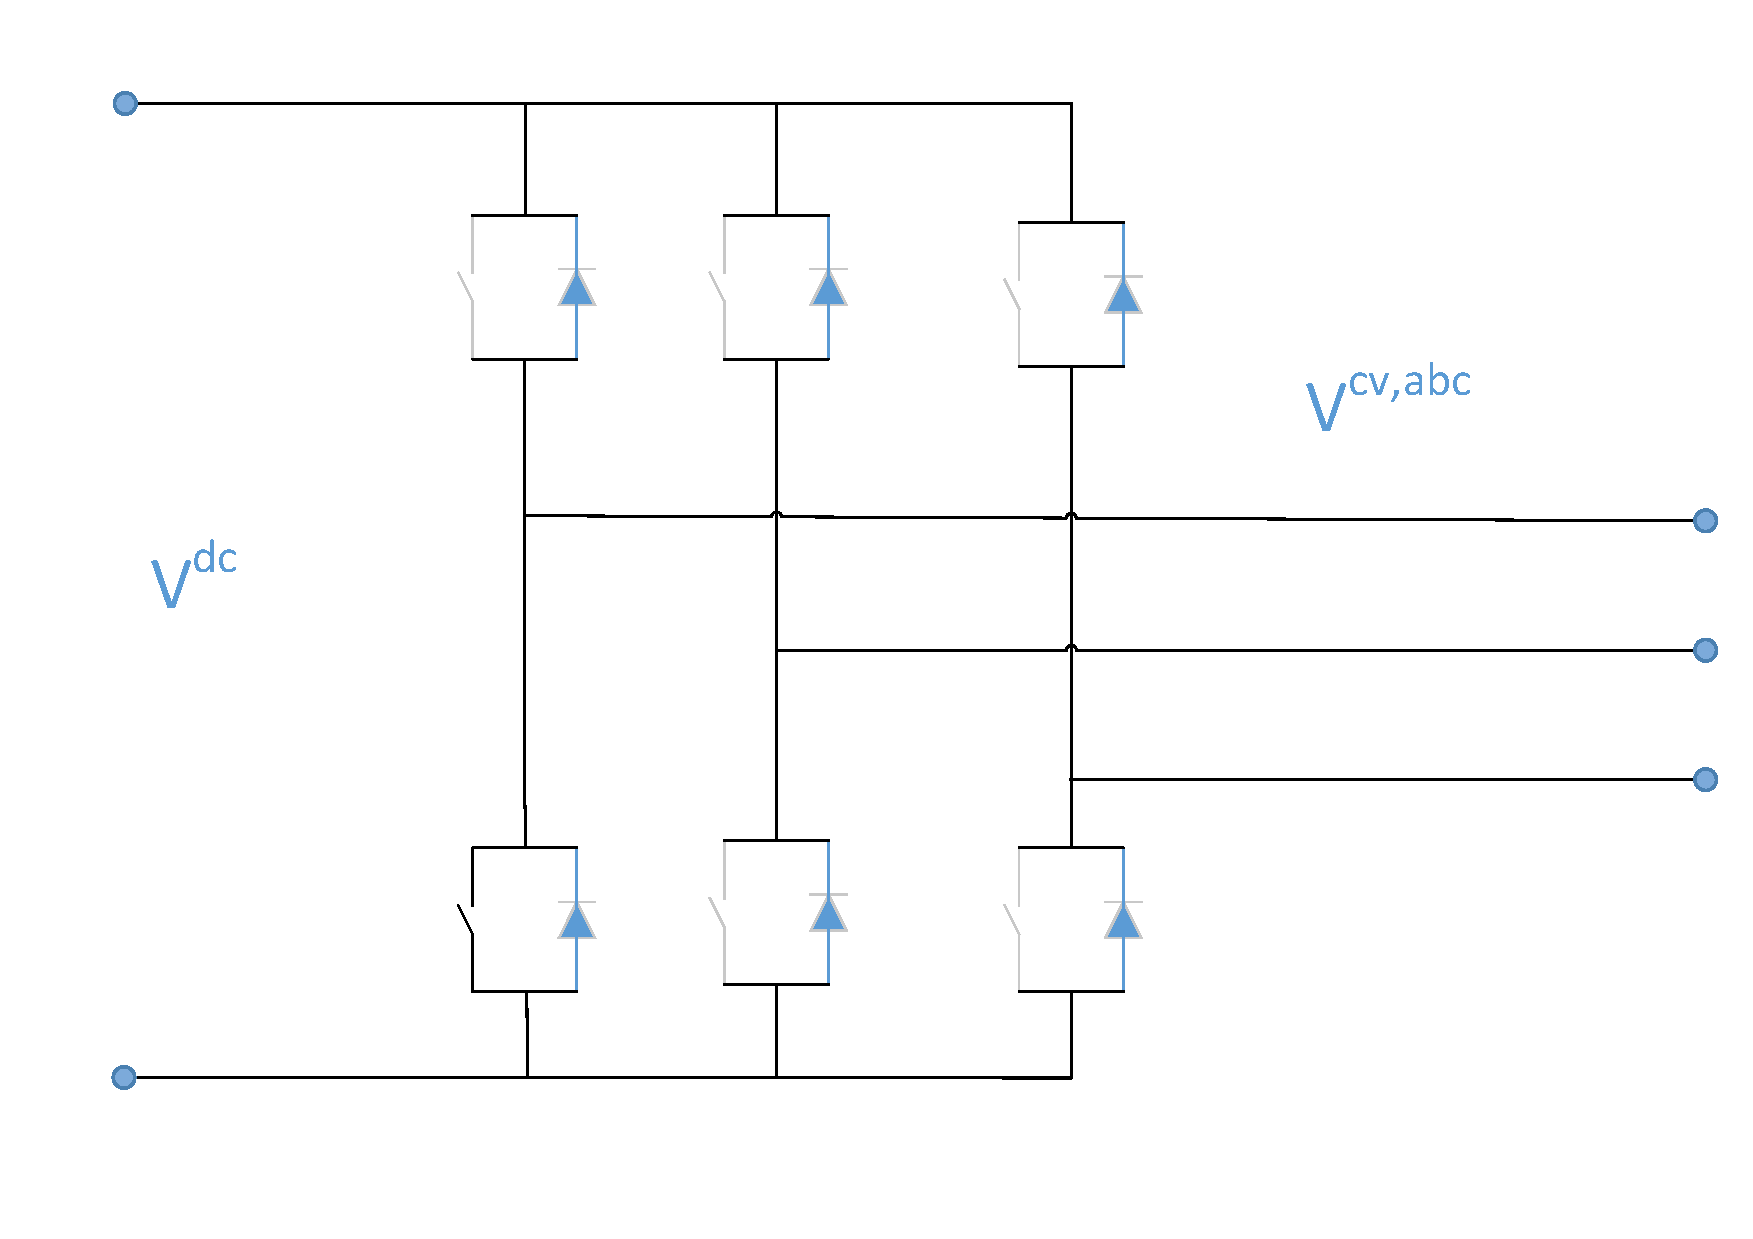
\includegraphics[width=\textwidth,height=\textheight,keepaspectratio]{Figures/Inverter.pdf}
    \caption{An inverter without the necessary filters on the AC or DC-side, (Inspired by \cite{Suul_electro_presentation_1})}
    \label{fig:PWM}
\end{figure}{}
In order to make different voltages on a line, a \gls{PWM} can only keep a connect a voltage to a high or a low voltage. The operates on short periods, where a certain fraction of that period is spent with a line connected to the high voltage, and the rest of the time, connected to the low one. This results in a voltage that jumps between two extremes at least once per period. In order to make a sine-wave the sluggishness of a RLC-circuit is used to make the voltage appear somewhat more smooth, and follow something that resembles more what the desired voltage should be. 

\begin{figure}
    \centering
    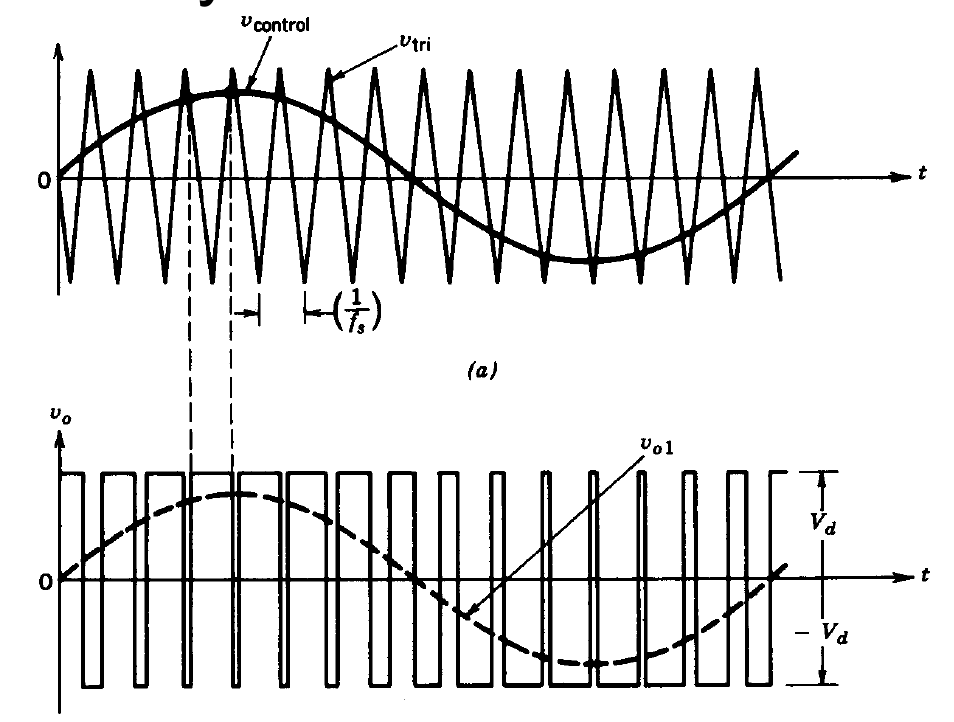
\includegraphics[width=\textwidth,height=\textheight,keepaspectratio]{Figures/PWM_response.png}
    \caption{Output-voltage from \gls{VSC}, given voltage reference and a low-pass filter \cite{Suul_electro_presentation_1}}
    \label{fig:PWM_response}
\end{figure}{}

The reference is usually in periodic intervals, and is given by the duty-cycle. The duty cycle is how long the voltage is high over a period. For a gate to be high, the upper gate of the inverter has to be open, while the lower one has to be closed. And it is the opposite to get a low voltage. 


\section{Park- and Clarke transformation and rotating reference frames}
\label{sec:rotating_reference_frame}
A normal three-phase AC current usually follows three sinusoidal waves that have a \ang{120} phase difference between each other. 

\begin{equation}
\begin{aligned}
    \label{eq:three_phase}
        V_a &= \hat{V}_a \cdot \sin{(\omega t + \phi )}\\
        V_b &= \hat{V}_b \cdot \sin{(\omega t + \phi + \frac{2\pi}{3} )}\\
        V_c &= \hat{V}_c \cdot \sin{(\omega t + \phi - \frac{2\pi}{3} )}
    \end{aligned}
\end{equation}
\begin{equation}
    V_{abc} = 
    \begin{pmatrix}
        V_a \\ 
        V_b \\ 
        V_c
    \end{pmatrix}
\end{equation}{}
If the system is balanced, the three voltages will always add up to 0. This means that we have a three-dimensional representation of the electrical lines, where one dimension is redundant. We can reduce the number of dimensions in a three-phased system by performing the Clarke-transformations, which rotates the reference-frame in such a way that one of the axis represents a scaled sum  of all three phases.  \cite{Clarke_transform_source}. Deriving the rotation-matrix is somewhat difficult, but the resulting rotation matrix will represent the Clarke-transformation from the $abc$ frame to the $\alpha\beta 0$ frame. 


\begin{equation}{}
    \label{eq:Clarke_transform}
    V_{\alpha\beta 0} = \frac{2}{3}
    \cdot
    \begin{bmatrix}
        1                   & -\frac{1}{2}          & -\frac{1}{2} \\
        0                   & \frac{\sqrt{3}}{2}    & -\frac{\sqrt{3}}{2} \\
        \frac{1}{\sqrt{2}}  & \frac{1}{\sqrt{2}}    & \frac{1}{\sqrt{2}}
    \end{bmatrix}
    V_{abc}
\end{equation}{}


\begin{figure}
    \centering
    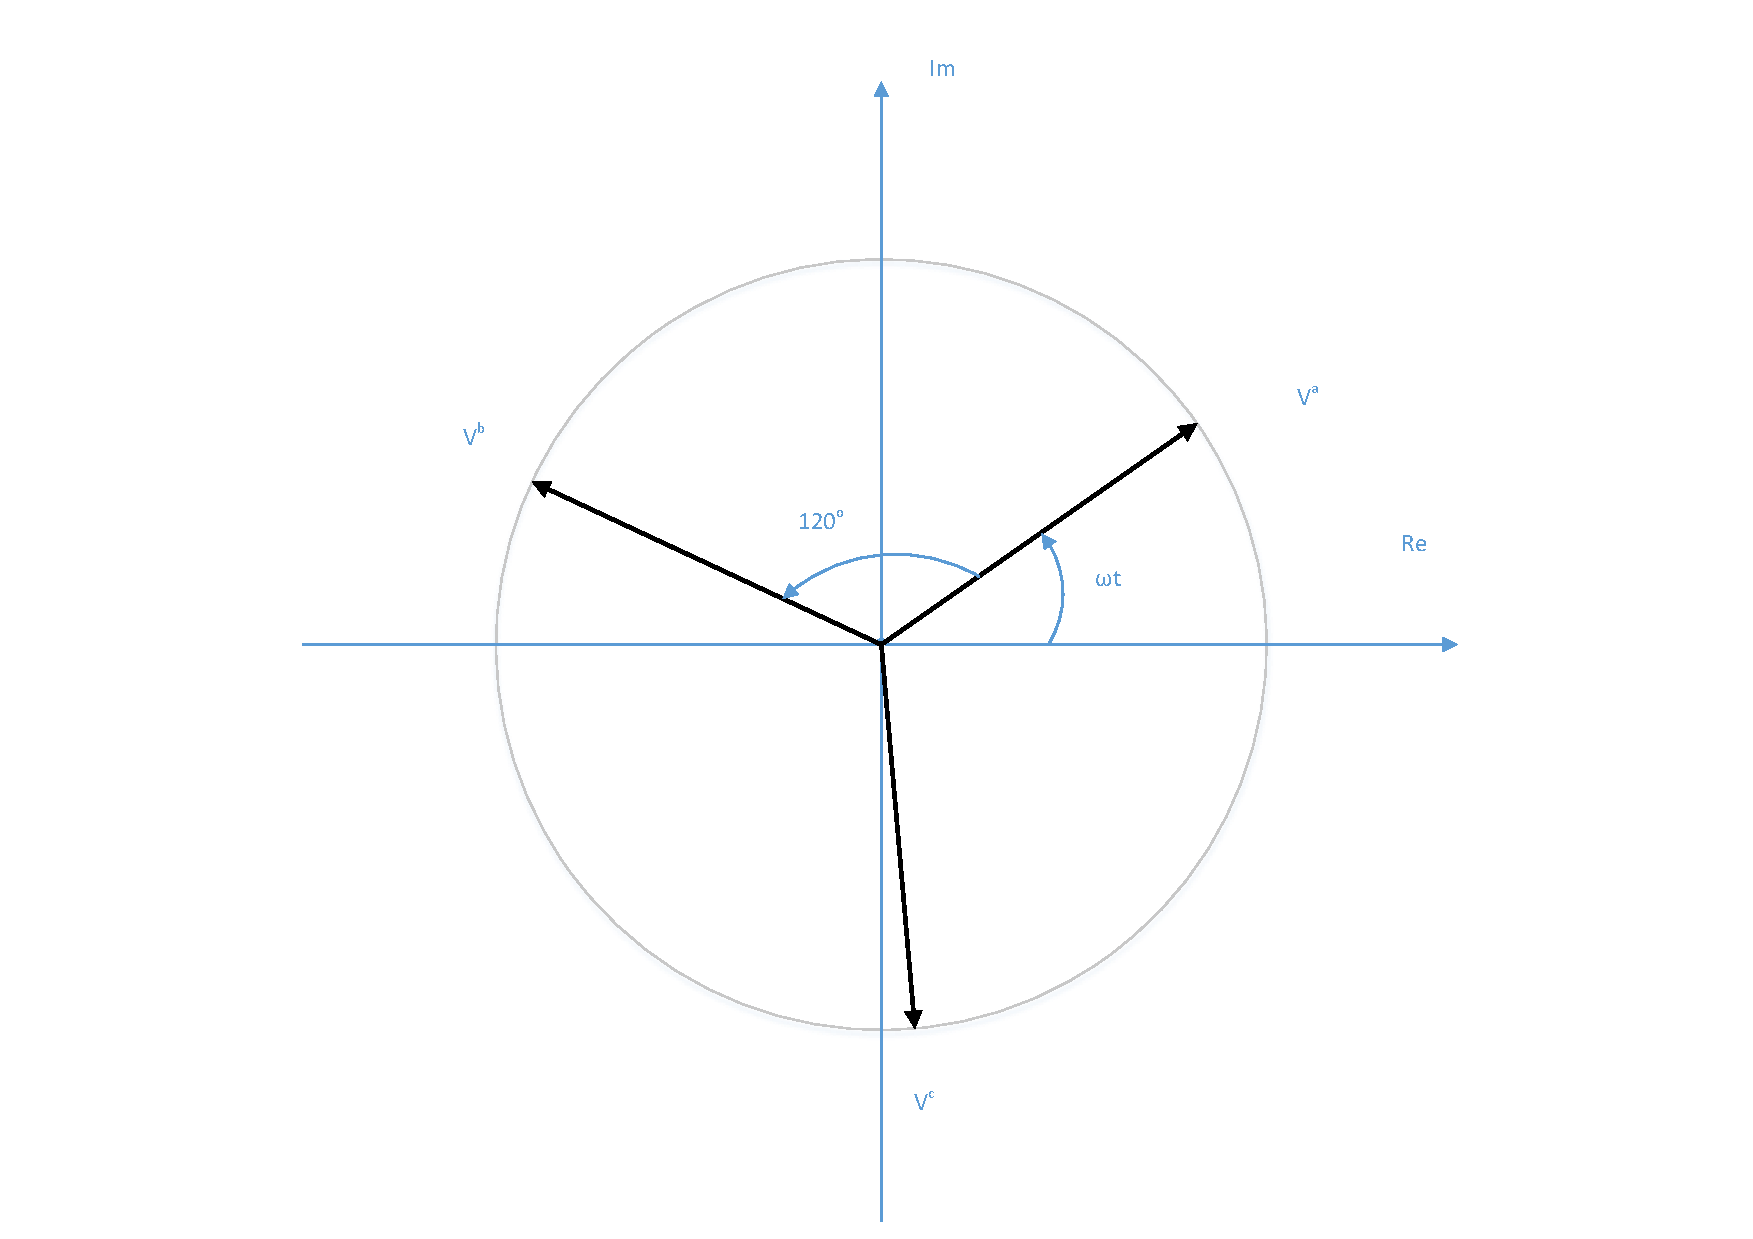
\includegraphics[width=\textwidth,height=\textheight,keepaspectratio]{Figures/Untransformed_phase.pdf}
    \caption{A representation of the three-phase system in the complex plane, when following the abc-reference frame}
    \label{fig:Current_circle}
\end{figure}


The Park transformation consists of rotating the $\alpha$ and $\beta$ axes by some arbitrary frequency. something within this reference frame has the same angular velocity as the rotation, it will be perceived  as a DC-current in the dq0- reference frame.  When looking at the transformation in  \Cref{fig:Current_circle}, it can be seen that if all components of the three-phase voltage are represented as orthogonal complex numbers along some circle.




\begin{figure}
    \centering
    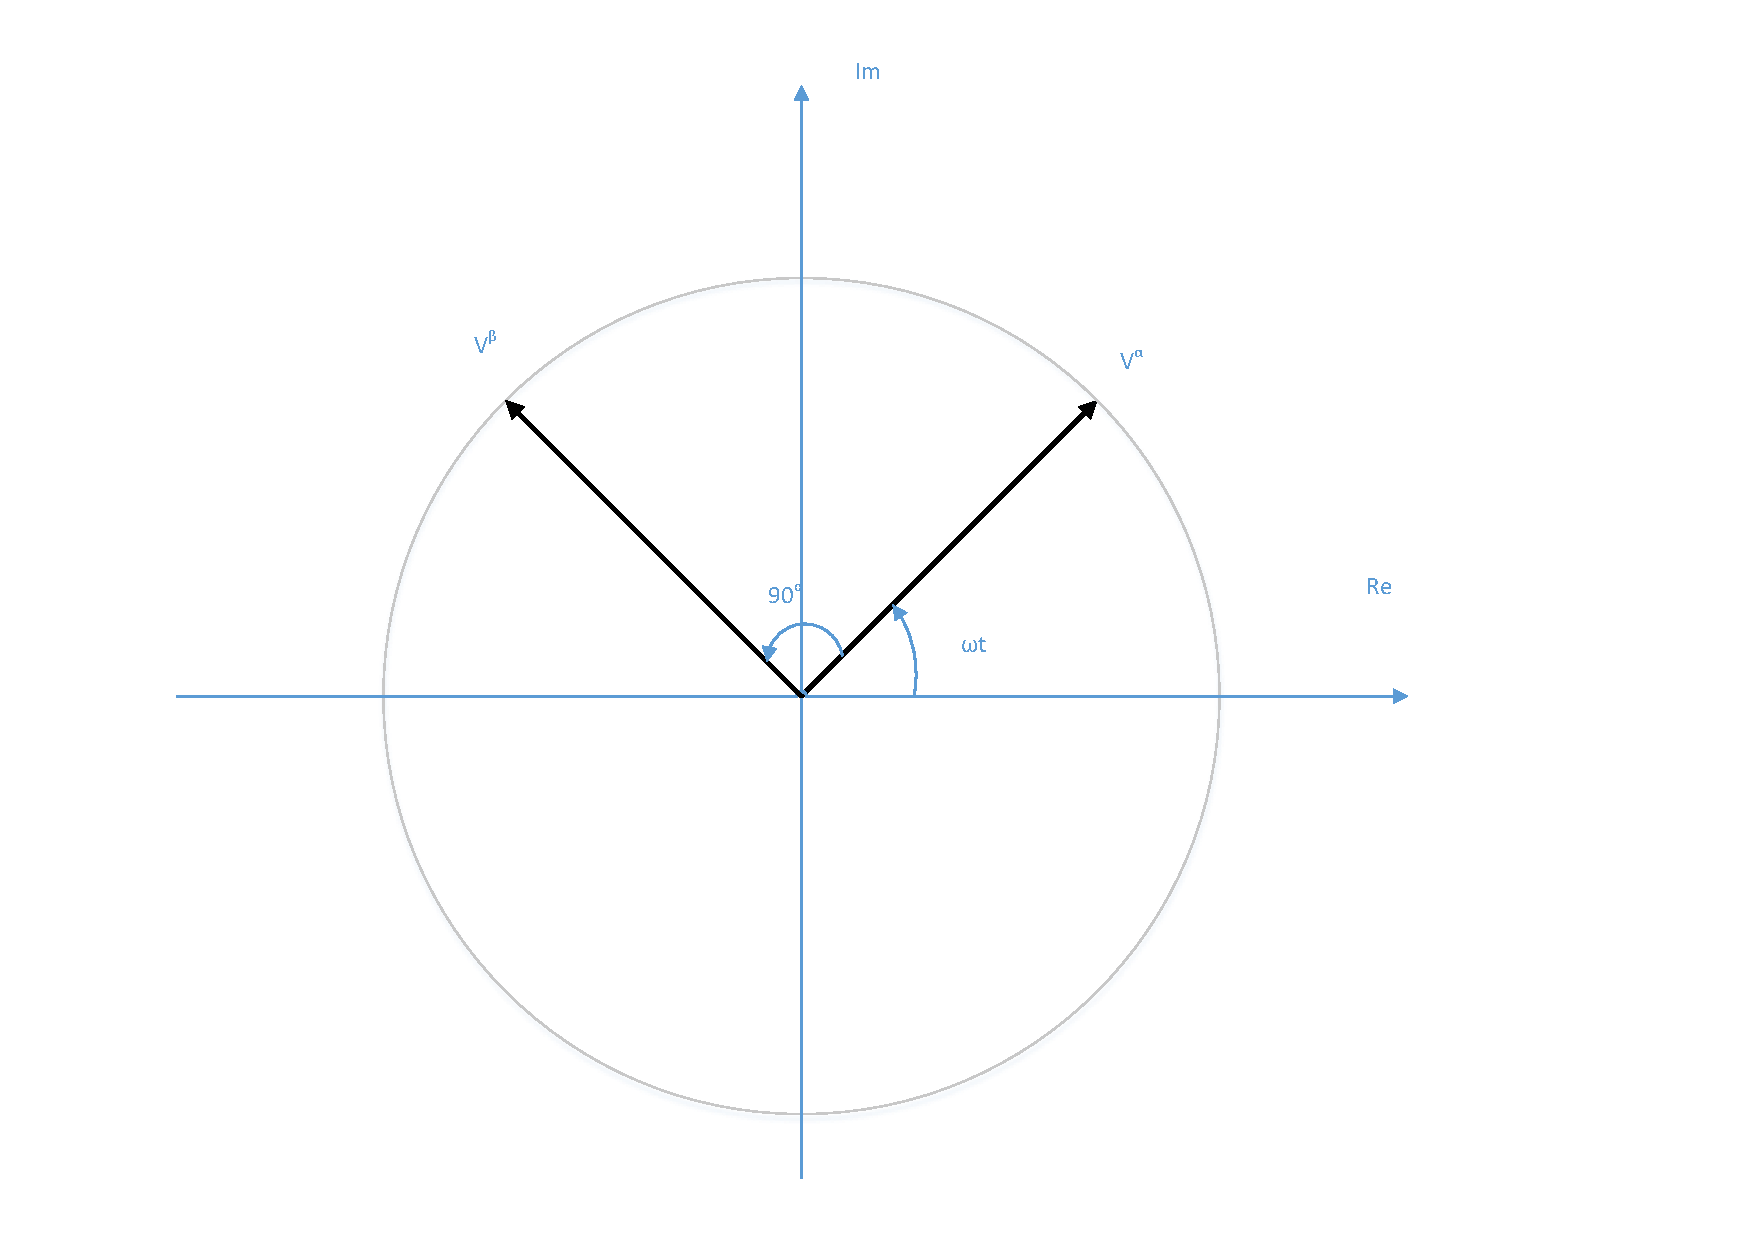
\includegraphics[width=\textwidth,height=\textheight,keepaspectratio]{Figures/Clarke_transformed.pdf}
    \caption{$\alpha$ and $\beta$ after the Clarke transformation. The phases are rotating $90^{\circ}$ from each other}
    \label{fig:First_clarke_transformation}
\end{figure}

\begin{figure}
    \centering
    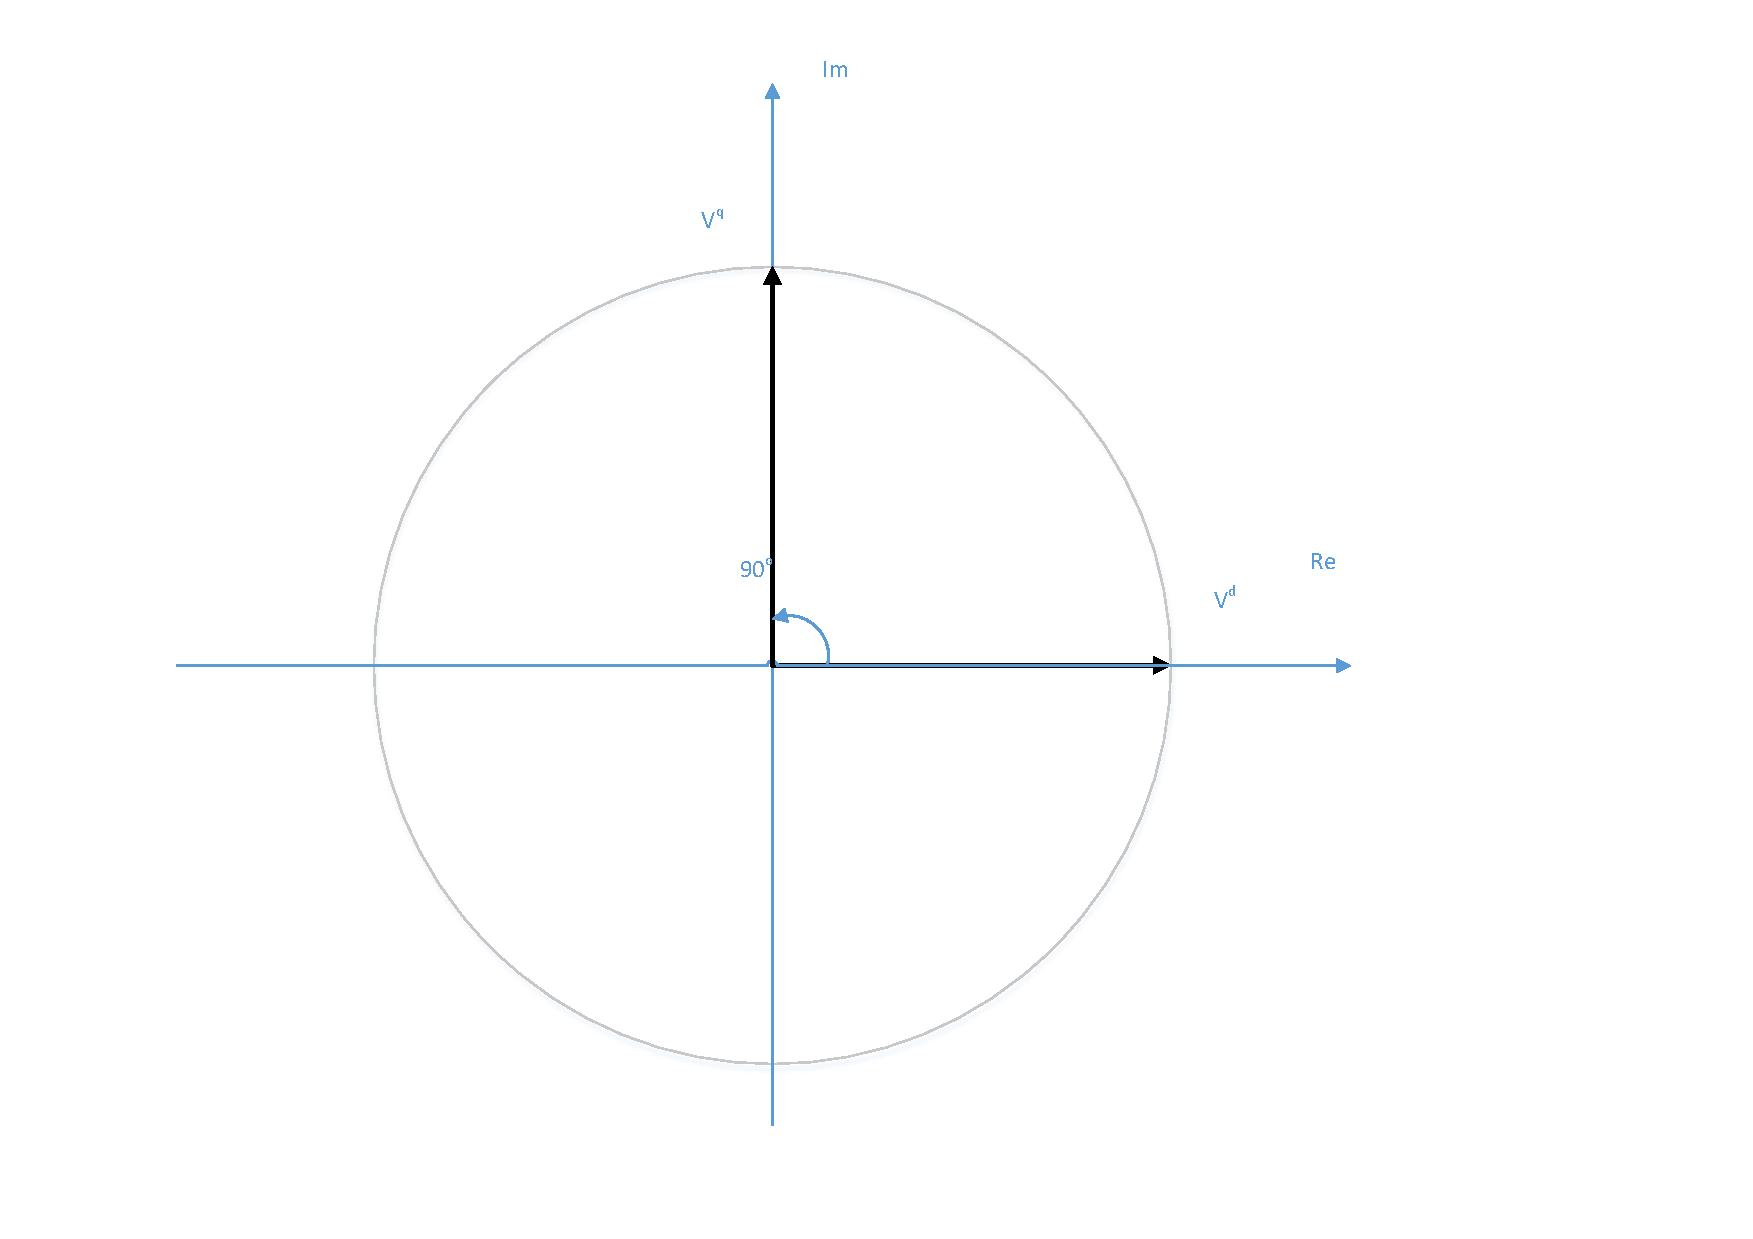
\includegraphics[width=\textwidth,height=\textheight,keepaspectratio]{Figures/Park_transformed.pdf}
    \caption{$d$ and $q$ after the Park transformation. The current-vectors no longer rotate in the complex plane if they had the same angular frequency as the transformation}
    \label{fig:Park_transformed}
\end{figure}

The vectors for abc, can be seen as rotating with an angular velocity $\omega$ as time passes, and if the value along the $\alpha$-axis is seen as the real value, while the value along the $\beta$ axis is seen as the imaginary one, the rotation 
\begin{equation}
    R_{park} = \begin{bmatrix}
       \cos{\left(\theta\right)} & \sin{\left(\theta\right)} \\
       -\sin{\left(\theta\right)} & \cos{\left(\theta\right)}\\

    \end{bmatrix}
\end{equation}

can be seen as a multiplication with $e^{-j\theta}$. Thus, if theta is the same as $\omega t$, the angle of $V_{dq} = R_{park}V_{\alpha\beta}$ will always remain constant, and the ac-voltage is observed as a DC-voltage. 

The Clarke, and the Park transformation can be combined into the DQZ-transformation. 

\begin{equation}
 \sqrt{\frac{2}{3}}\begin{bmatrix}
   \cos{\left(\theta\right)}
      & \cos{\left(\theta - \frac{2\pi}{3}\right)}
      & \cos{\left(\theta + \frac{2\pi}{3}\right)} \\
   -\sin{\left(\theta\right)}
      & -\sin{\left(\theta - \frac{2\pi}{3}\right)}
      & -\sin{\left(\theta + \frac{2\pi}{3}\right)} \\
   \frac{\sqrt{2}}{2}
      & \frac{\sqrt{2}}{2}
      & \frac{\sqrt{2}}{2}
\end{bmatrix}
\end{equation}{}


The dq0- transformation is a non-linear transformation that makes it possible to observe the frequency and the amplitude of an AC-voltage of one specific frequency as something constant. This makes it possible view the system as a time-invariant one. This is a necessary condition if a normal PI-regulator is supposed to be able to control the system towards zero deviation from the reference. 


    
\section{Exact response from a Polynomial input }    
\todo[inline]{Bedre tittel på denne delen}
\label{sec:finding_response_from_polynomial_inputs}
$e^{\Vec{A}t}$ is defines as 
\begin{equation}
    e^{\Vec{A}t} \triangleq  \sum_{n=0}^\infty A^n \frac{t^n}{n!}
\end{equation}{}
To show that the time-response for any $\Vec{x}(t)$, as long as $\Vec{u}(t)$ is constant, we approximate $\Vec{x}(t)$ by a Taylor series. 
\begin{equation}
    \dot{\Vec{x}} = \Vec{A}\Vec{x} + \Vec{Bu}
\end{equation}{}
    
\begin{equation}
    \ddot{\Vec{x}} = \frac{d}{dt} \left( \Vec{A}\Vec{x} + \Vec{Bu} \right) = \Vec{A}( \Vec{Ax}+ \Vec{Bu}) + \Vec{B \dot{u} }
\end{equation}{}

\begin{equation}
    \frac{d^n\Vec{x}}{dt^n} = \Vec{A}^nx + \sum_{m=1}^n \Vec{A}^{n-m}\Vec{B}\frac{d^{m-1}\Vec{u}}{dt^{m-1}}
\end{equation}{}

\begin{figure}
    \centering
    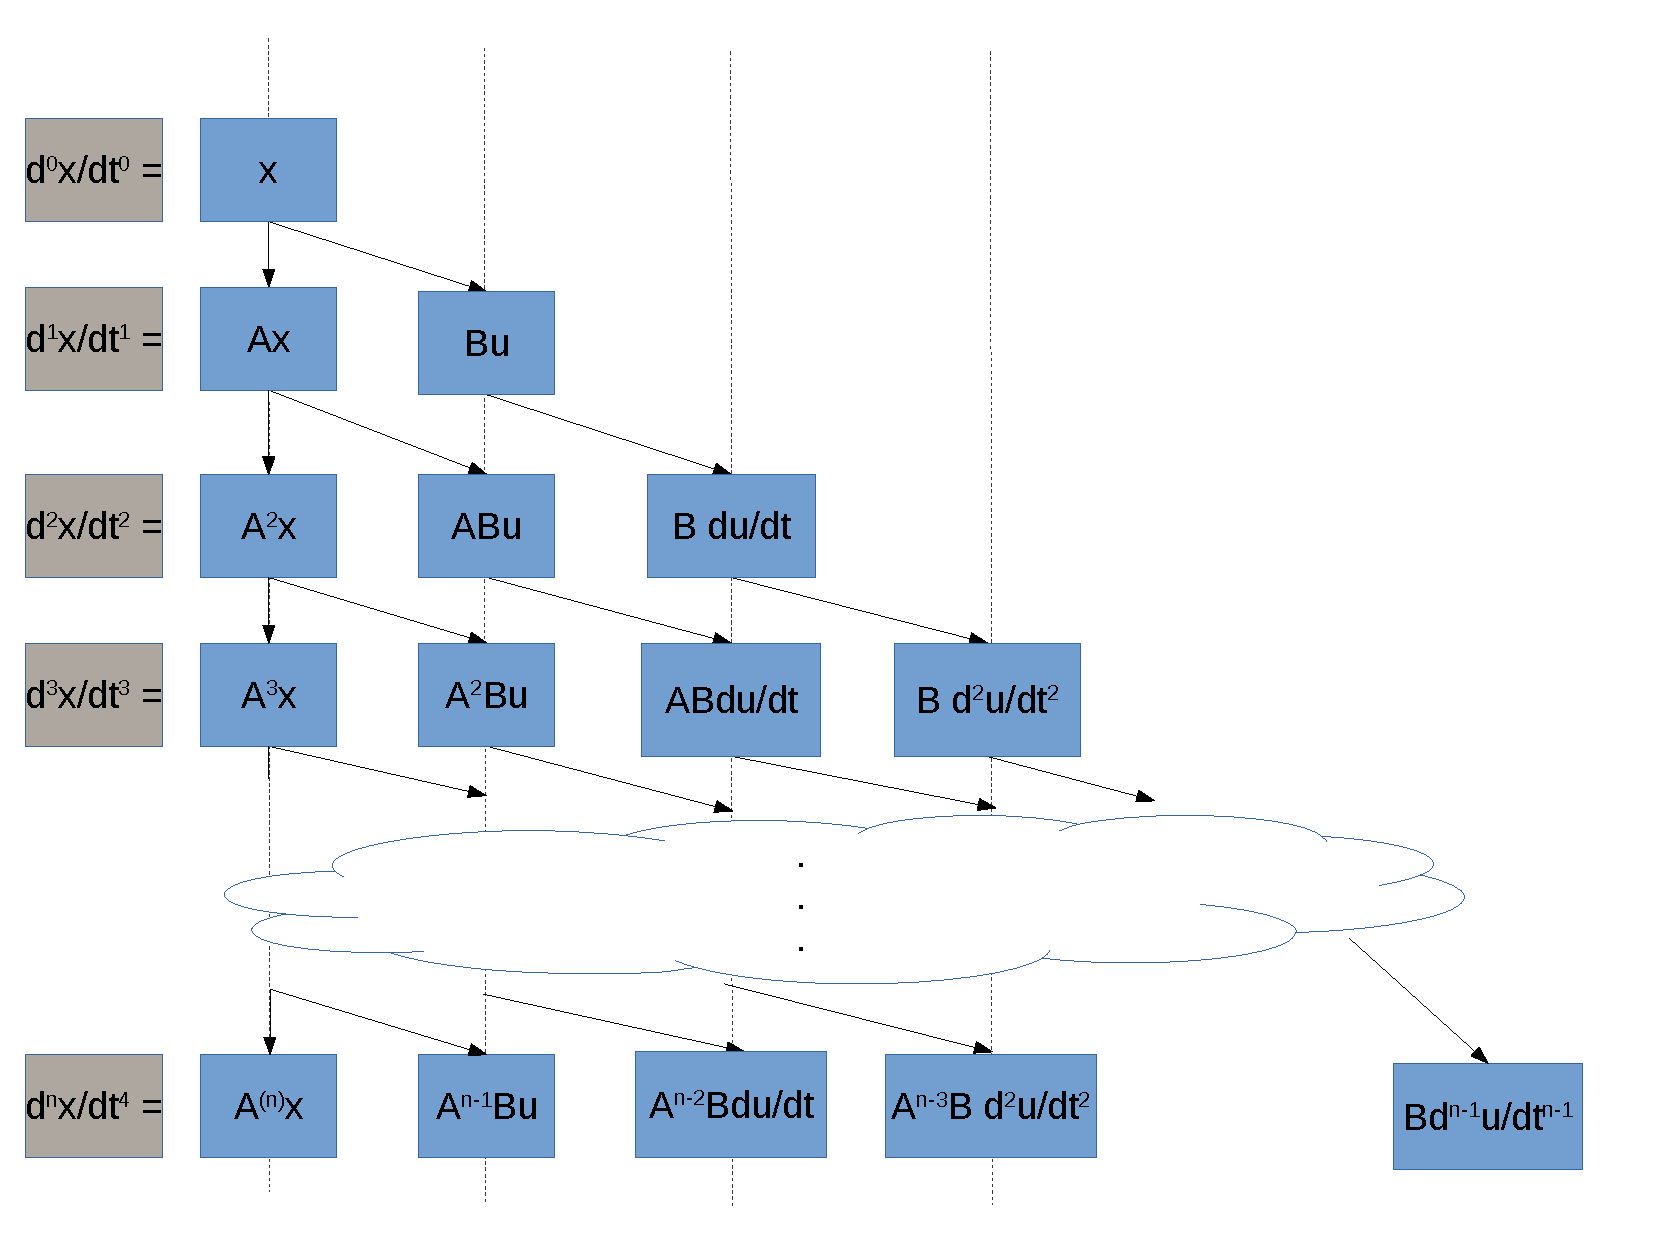
\includegraphics[width=\textwidth,height=\textheight,keepaspectratio]{Figures/Derivasjons_figur.pdf}
    \caption{Structure of the nth derivative of x}
    \label{fig:derivative_figure}
\end{figure}
Which has the same structure as \cref{fig:derivative_figure}

If $\Vec{u}$ has a finite number of derivatives, it will be possible to use the Taylor-series of $e^{\Vec{A}t}$ to give the exact series that are proportional to any derivative of $\Vec{u}$. Each step from $n > m$ in the sequence can be expressed as 
\begin{equation}
    \Vec{A}^{n-m}\Vec{B}\frac{d^{m-1}\Vec{u}}{dt^{m-1}}
\end{equation}{}

Which means, that if we can subtract the first m terms from $\Vec{A}^{-m-1}e^{\Vec{A}t}$, it is possible to express $\Vec{x}(t)$ as 

\begin{equation}
    \Vec{x}(t) = e^{\Vec{A}t}\Vec{x(0)} + \sum_{m=0}^M A^{-m-1}\left( e^{\Vec{A}t}\Vec{x(0)} - \sum_{i=0}^{m}\frac{\Vec{A}^i}{i!} \right)\Vec{B}\frac{d^m\Vec{u}}{dt^m}(0)
\end{equation}{}
where $M$ is the highest order derivative of $\Vec{u}$. This means that it is possible to get an exact solution of a linear system for any input u, that can be expressed as a finite polynomial. 

If the time-step $t=T_s$ is known in advance, it is possible to make a matrix $e^{\Vec{A}T_s}$ in advance, which can give an exact solution for any initial state. The response from the inputs will have to be a sum of products different matrices and the derivatives of $\Vec{u}$, where each matrix is constant, possibly different for each derivative.


But whenever somebody solves linear systems, $M$ is almost always equal to 1, which gives the simpler equation. 

\begin{equation}
        \Vec{x}(t) = e^{\Vec{A}t}\Vec{x(0)} + \Vec{A}^{-1}\left( e^{\Vec{A}t}\Vec{x(0)} - \Vec{I} \right)\Vec{u}
\end{equation}{}

But, we will sadly need the general solution for if the system matrix has Jordan-blocks with eigenvalues equal to 0, that are larger than $(1x1)$

\todo[inline]{Gjør denne litt mer presis}
    



\section{Finding \texorpdfstring{$e^{\Vec{A}t}$}{}  when A is  defective}
\label{sec:finding_eAt_when_A_is_defective}
Normally, when trying to find the exact solution of a linear system, given some initial values, it is done by diagonalising the matrix $\Vec{A}$, and then solving the much simpler set of first order equations that don't interact with each other. But, not all matrices are diagonalisable. One such example is: 
\begin{equation}
    A_{deg} = 
    \begin{bmatrix}
        0 & 1 \\ 
        0 & 0 
    \end{bmatrix}
\end{equation}
Luckily, all matrices can be written on Jordan-form \cite[Chp 1]{Triangle_inequality_source}, where each vector in the basis satisfies. 
\begin{equation}
    (\Vec{A}- \lambda_i \Vec{I})\Vec{e_i} = 0
\end{equation}
or
\begin{equation}
    \exists e_j s.t  (\Vec{A}- \lambda_i \Vec{I})\Vec{e_i} = \Vec{e_j}
\end{equation}
In these cases, the matrix $\Vec{A}$ can be written on a form $\Vec{Q^{-1} J Q}$. where $\Vec{J}$ is a block-diagonal matrix, where each block has a diagonal corresponding to an eigenvalue, and a superdiagonal with elements equal to 1. As a result, each Jordan-block can be solved separately. 
\begin{equation}
    \Vec{J_i} = 
    \begin{bmatrix}
        \lambda_i & 1         & 0      & \cdots &0          &0\\
        0         & \lambda_i & 1      &\cdots  & 0         &0\\
        \vdots    & \vdots    & \ddots & \ddots & \vdots    & \vdots \\
        \vdots    & \vdots    & \ddots & \ddots & \vdots    & \vdots \\
        0         & 0         & 0      & \cdots & \lambda_i & 1 \\
        0         & 0         & 0      & \cdots & 0         & \lambda_i \\
    \end{bmatrix}
\end{equation}

Each Jordan-block can be solved by first solving the independent equation, and working upwards from there. Take note that we will break notation and refer to the lowest state in the Jordan-block as $q_1$ and work our way upwards to $q_n$. 
\begin{equation}
    q_1 = \lambda_i q_1 
\end{equation}
Which gives an expression $q_1(t)= q_1(0) e^{\lambda_i t}$. The following element will be the solution of 
\begin{equation}
    q_2 = \lambda_i q_2 + e^{\lambda_i t}q_1(0)
\end{equation}
Which can be solved by $q_2(t)  = e^{\lambda_i t}q_2(0) + t e^{\lambda_i t}q_i(0)$. As we can see, a pattern emerges quickly, where the product-rule together with an an exponential is used to describe both a state $q_i$ and its predecessor $q_{i+1}$. But, since the derivative of $t^n = nt^{n-1}$, a the result will also have to be multiplied by a constant. The result is something along the lines of: 
\begin{equation}
    q_{j}(t) = q_j(0)e^{\lambda_i t} + \sum_{k=1}^n \frac{t^{k}}{k!}q_{j-k}(0)e^{\lambda_i t} 
\end{equation}
The resulting matrix for the solution becomes. 
\begin{equation}
    e^{\Vec{J_i} t } = e^{\lambda_i t} 
    \begin{bmatrix}
        1      & \frac{t}{1!} & \frac{t^2}{2!} & \frac{t^3}{3!} &\cdots  & \frac{t^{n-1}}{(n-1)!} & \frac{t^n}{n!}\\
        0      & 1            & \frac{t}{1!}   &\frac{t^2}{2!}  & \cdots & \frac{t^{n-2}}{(n-2)!} & \frac{t^{n-1}}{(n-1)!}\\
        0      & 0            & 1              & t              & \cdots & \frac{t^{n-3}}{(n-3)!} & \frac{t^{n-2}}{(n-2)!} \\
        \vdots & \vdots       & \vdots         &\vdots          & \ddots & \vdots                   & \vdots \\
        0      & 0            & 0              & 0              & \cdots & 1                        & \frac{t}{1!} \\
        0      & 0            & 0              &0               & \cdots & 0                        & 1
    \end{bmatrix}
\end{equation}
This also means that $e^{\Vec{J_i} t }$ is a solution of the Taylor-series including $\Vec{J}$. And since $\Vec{A}= \Vec{Q^{-1}JQ}$, the Taylor-series of A will mostly contain cancellations between $\Vec{Q}$ and $\Vec{Q}^{-1}$, making each term into $\Vec{\frac{t^n}{n!} Q^{-1}J^nQ}$. This means that the solution for $e^{\Vec{J}t}$
\begin{equation}
    e^{\Vec{A}t} = \Vec{Q}^{-1}e^{\Vec{J_i} t }\Vec{Q} 
\end{equation}

As a result, it is possible to find the exact response for a linear system. Even if the number of eigenvectors is too small to cover the entire space. 



\section{Finding exact step-response when A is non-invertible}
\label{sec:solving_for_uninvertible_matrices}
When finding the system-response for constant input, it is usually found by using the expression
\begin{equation}
    \Vec{A}^{-1} \left( e^{\Vec{A}t} - \Vec{I}\right)
\end{equation}
But if $\Vec{A}$ has any eigenvectors that are equal to 0, then $\Vec{A}$ will not be invertible. As a result, this method will not work directly. On the other hand, from the analysis in \cref{sec:finding_response_from_polynomial_inputs}, we saw that the input-response is still given by a Taylor-series, so it definitely exists. 
If the system is written on Jordan canonical form the problem is solvable. We can invert  and solve normally for any block where $\lambda_i \neq 0$. In the case of the subspace where $\lambda_i =0$, set it the non-existent inverted Jordan-block to be 0, so that it can be solved later. We call this pseudo-inverted matrix $J^{-1}_{pi}$.
The interesting parts about Jordan-blocks when the eigenvalues are 0 is that each state will act as a pure integrator with respect to something. As a result, the input-response for the sub-space will act very similarly to the impulse response for a system with eigenvalues equal to 0. The only difference is that the first (constant) state is replaced by a constant input instead. 

Therefore, if the Jordan-block looks like this 

\begin{equation}
    \begin{bmatrix}{}
    \lambda_i & 1 & 0 &\dots &\dots & 0 & 0  \\
    0 & \lambda_i & 1 & \dots &\dots & 0 & 0 \\
    \vdots & \vdots & \vdots & \ddots & \ddots & \vdots & \vdots &\\
    \vdots & \vdots & \vdots & \ddots & \ddots & \vdots & \vdots &\\
    0 & 0 & 0 & \dots  & \dots & \lambda_i & 1 \\ 
    0 & 0 & 0  & \dots & \dots & 0 & \lambda_i \\
    \end{bmatrix}
\end{equation}{}

and $\lambda_i =0$, the exact solution will look like: \\

\begin{equation}
    \gls{step_resp}_{\lambda=0}(t) = 
\begin{bmatrix}{}

t & \frac{t^2}{2!} & \frac{t^3}{3!} &\dots &\dots & 0 & \frac{t^n}{n!} \\
 0 & t & \frac{t^2}{2!} & \dots &\dots & 0 & \frac{t^{n-1}}{(n-1)!} \\
 
 \vdots & \vdots & \vdots & \ddots & \ddots & \vdots & \vdots\\
 
 \vdots & \vdots & \vdots & \ddots & \ddots & \vdots & \vdots\\
 
 0 & 0 & 0 & \dots & \dots & t & \frac{t^2}{2!} \\
 
 0 & 0 & 0 & \dots & \dots & 0 & t \\
\end{bmatrix}
\end{equation}{}
So if a specialised block-diagonal matrix $\gls{step_resp}_{non\_inv}$, where all values are 0, except for the block $\gls{step_resp}_{\lambda=0}(t)$ for the subspace that belongs to the singular Jordan-block. 


\begin{equation}
    \Vec{x}(t) = e^{\Vec{A}t}\Vec{x}(0) + \Vec{Q}^{-1}\Vec{J}^{-1}_{pi}\Vec{Q}(e^{\Vec{A}t}\Vec{x} - \Vec{I})\Vec{Bu} + \gls{step_resp}_{non\_inv}(t) \Vec{Bu}
\end{equation}{}

If the time-step is a known constant, then the two matrices from the input can be combined into one constant matrix. 



\section{Differentiating the step-response of a non-invertible system}
\label{sec:differentiating_step_response_from_input}
Normally
\begin{equation}
    \frac{d \gls{step_resp}}{d \rho} = \frac{d\Vec{A^{-1}}}{d \rho} \left( e^{\Vec{A}t} - \Vec{I}\right)\Vec{B} + \Vec{A}^{-1} \left( \frac{de^{\Vec{A}t}}{d\rho}\right)\Vec{B} +  \Vec{A^{-1}} \left( e^{\Vec{A}t} - \Vec{I}\right)\frac{d\Vec{B}}{d\rho}
\end{equation}
This solution is obviously not possible if A can't be inverted, so an alternative has to be found. In this project, no general solution was found for this problem. But, if the subspace, made out of generalised eigenvectors, with eigenvalues equal to 0 is unaffected by $\rho$, then it is possible perform a change of basis, by using a matrix $\Vec{Q}$

Which leads to 
\begin{equation}
    \Vec{Q}^{-1}\Vec{q} = \Vec{x}
\end{equation}
\begin{equation}
    \dot{\Vec{q}} = \Vec{QAQ}^{-1}\Vec{q} + \Vec{QB}\Vec{u}
\end{equation}

If $\Vec{Q}$ is chosen properly, it is possible to separate the system into a well-behaved part, and the part where the eigenvalues are equal to 0.
\begin{equation}
    \dot{\Vec{q}}=
    \begin{bmatrix}
        \Vec{A}_{sub} & \Vec{A}_{1,2}\\
        \Vec{0} & \Vec{J}_{\lambda=0}
    \end{bmatrix}
    \Vec{q}
    + 
    \begin{bmatrix}
        \Vec{B}_{sub}\\
        \Vec{B}_{\lambda=0}
    \end{bmatrix}
    \Vec{u}
\end{equation}
Because of this separation, $\Vec{q}$ can be split into two parts
\begin{equation}
    \Vec{q}= \begin{bmatrix}
        \Vec{q_{sub}}\\
        \Vec{q}_{\lambda =0}
    \end{bmatrix}
\end{equation}
\todo[inline]{Bedre navn på koblingen mellom dem}


One transformation that can split the system into two parts, like this is the transformation into Jordan-canonical form. But, in order to make the differentiation simpler, the same transform is used, even after $\rho$ might have changed the bases of $\Vec{A}_{sub}$. This makes the differentiation a lot easier. 
\noindent
If $\Vec{B}_{\lambda=0}$ is unaffected by $\rho$, then $\Vec{q}_{\lambda=0}$ can be solved independently. Each Jordan-block will have a solution on the form: 
\begin{equation}
    \gls{step_resp}_{Jordan\_block} = 
    \begin{bmatrix}
        t & \frac{t^2}{2!} & \cdots & \frac{t^{n}}{n}\\
        0 & t  & \cdots & \frac{t^{n-1}}{(n-1)!}\\
        \vdots & \vdots & \ddots & \vdots & \\
        0 & 0 & \cdots & t
    \end{bmatrix}    
\end{equation}
Where n is the number of linearly independent generalised eigenvectors that result from an ordinary eigenvector (including itself). As a result, \gls{step_resp} will be a block-diagonal matrix with one or several blocks like $\gls{step_resp}_{Jordan\_block}$, but of potentially different sizes.

Since the matrix $\Vec{A}_{sub}$ now is guaranteed to only have eigenvalues that are different from 0, it is guaranteed to be invertible\cite{LinSys_boken,Triangle_inequality_source}. As a result, it is possible to use the methods from \cref{sec:finding_response_from_polynomial_inputs} by viewing the states in $\Vec{q}_{\lambda =0}$ as inputs  to $\Vec{q_{sub}}$.

\begin{equation}
    \Vec{\dot{q}_{sub}} = \Vec{A}_{sub} \Vec{q_{sub}} + \left(\Vec{A}_{1,2}\gls{step_resp}_{\lambda=0}\Vec{B}_{\lambda=0} + \Vec{B}_{sub} \right)\Vec{u}
\end{equation}

Afterwards, the technique from \cref{sec:finding_response_from_polynomial_inputs} can be used to get an absolute monster. Notice that the response from initial conditions in $\Vec{q}_{\lambda =0}$ is the same as $\frac{d \gls{step_resp}}{dt }$. 
\begin{dmath}
    \Vec{q}_{sub}(t) = e^{\Vec{A}_{sub} t}\Vec{q}_{sub}(0) + \Vec{A}_{sub}^{-1}\left(e^{\Vec{A}_{sub} t} -\Vec{I}\right)\Vec{B}_{sub} \\+ \sum_{i=0}^n \Vec{A}_{sub}^{-i-1}\left( e^{\Vec{A}_{sub} } - \sum_{k=0}^{i} \frac{\Vec{A}^k_{sub}}{k!}\right) \left( \frac{d^i \gls{step_resp}_{\lambda=0}(0)}{dt^i} \Vec{B}_{\lambda=0}\Vec{u}(0) + \frac{d^{i+1} \gls{step_resp}_{\lambda=0}(0)}{dt^{i+1}} \Vec{q}_{\lambda=0}(0) \right) 
\end{dmath}

So, when setting up the system on matrix-form, it becomes: 

\begin{dmath}
    \Vec{q}(t) = 
    \begin{bmatrix}
        e^{\Vec{A}_{sub} t} & \sum_{i=0}^n \Vec{A}_{sub}^{-i-1}\left( e^{\Vec{A}_{sub} } - \sum_{k=0}^{i} \frac{\Vec{A}^k_{sub}}{k!}\right)\frac{d^{i+1} \gls{step_resp}_{\lambda=0}(0)}{dt^{i+1}} \\
        0 & \frac{d \gls{step_resp}_{\lambda=0}}{dt}
    \end{bmatrix}
    \begin{bmatrix}
        \Vec{q}_{sub}(0)\\
        \Vec{q}_{\lambda=0}(0)
    \end{bmatrix}\\
    + 
    \begin{bmatrix}
        \Vec{A}_{sub}^{-1}\left(e^{\Vec{A}_{sub} t} -\Vec{I}\right) &
        \sum_{i=0}^n \Vec{A}_{sub}^{-i-1}\left( e^{\Vec{A}_{sub} } - \sum_{k=0}^{i} \frac{\Vec{A}^k_{sub}}{k!}\right) \left( \frac{d^i \gls{step_resp}_{\lambda=0}(0)}{dt^i}  \right)  \\
        0 & \gls{step_resp}_{\lambda=0} 
    \end{bmatrix}
    \Vec{Q}\Vec{B}\Vec{u}
\end{dmath}

The response of $\Vec{q}$ can be translated back to $\Vec{x}$ to become
\begin{dmath}
    \Vec{x}(t) = 
    e^{\Vec{A}t}\Vec{x}(0)
    + 
    \Vec{Q}^{-1}
    \begin{bmatrix}
        \Vec{A}_{sub}^{-1}\left(e^{\Vec{A}_{sub} t} -\Vec{I}\right) &
        \sum_{i=0}^n \Vec{A}_{sub}^{-i-1}\left( e^{\Vec{A}_{sub} } - \sum_{k=0}^{i} \frac{\Vec{A}^k_{sub}}{k!}\right) \left( \frac{d^i \gls{step_resp}_{\lambda=0}(0)}{dt^i}  \right)  \\
        0 & \gls{step_resp}_{\lambda=0} 
    \end{bmatrix}
    \Vec{Q}\Vec{B}\Vec{u}
\end{dmath}

\section{Differentiation non-invertible matrices}
\label{sec:upper_bound_for_errors_in_noninvertible_systems}
As before, the given operations are only possible if there is no change in the where the eigenvalues are equal to zero. 
\begin{dmath}
    \Vec{x}(t) = 
    e^{\Vec{A}t}\Vec{x}(0)
    + 
    \Vec{Q}^{-1}
    \begin{bmatrix}
        \Vec{A}_{sub}^{-1}\left(e^{\Vec{A}_{sub} t} -\Vec{I}\right) &
        \sum_{i=0}^n \Vec{A}_{sub}^{-i-1}\left( e^{\Vec{A}_{sub} } - \sum_{k=0}^{i} \frac{\Vec{A}^k_{sub}}{k!}\right) \left( \frac{d^i \gls{step_resp}_{\lambda=0}(0)}{dt^i}  \right)  \\
        0 & \gls{step_resp}_{\lambda=0} 
    \end{bmatrix}
    \Vec{Q}\Vec{B}\Vec{u}
\end{dmath}

Differentiating this expression a matter of using the product-rule, as well as 
\begin{align}
    \frac{d \Vec{A}^{-1}}{dt} = \Vec{A}^{-1} \frac{d \Vec{A}}{dt}\Vec{A}^{-1}
\end{align}
and Taylor-series. The resulting differentiation will most likely not fit on the page. 
\subsection{Upper bound for the error}
The only term that can't be differentiated properly is $e^{\Vec{A}_{sub}}$ and  $e^{\Vec{A}}$. We will denote the difference between a true differentiation and an estimated one as. 
\begin{equation}
    \frac{ d \tilde{\mathbb{A} } }{d\rho } = \sum_{i=N}^\infty \sum_{k=1}^i \Vec{A}^{k-1}\frac{d \Vec{A}}{d \rho}\Vec{A}^{i-k}\frac{\left(T_s \right)^i }{i!}
\end{equation} 
Which is the difference between the derivative of the first N terms of the Taylor-series and the true derivative. 

As a result, when looking at the error from differentiating the step-response, the only terms that could not be differentiated are the differentiations in the product-rule that required the derivative of $e^{\Vec{A t}}$ the resulting error is :
\begin{dmath}
    \Vec{Q}^{-1}
    \begin{bmatrix}
                \Vec{A}_{sub}^{-1}\frac{ d \tilde{\gls{impulse_resp}_{sub} } }{d\rho } &
                \sum_{i=0}^n \Vec{A}_{sub}^{-i-1}\left( \frac{ d \tilde{\gls{impulse_resp}_{sub} } }{d\rho }\right) \left( \frac{d^i \gls{step_resp}_{\lambda=0}(0)}{dt^i}  \right)  \\
                0 & 0
    \end{bmatrix}\Vec{Q}\Vec{B}
    \label{eq:error_in_differentiation}
\end{dmath}
This is because terms, like $\Vec{B}$, $\Vec{A}^{n}$ and $\Vec{A}^{-n}$ can all be differentiated exactly, while $\Vec{Q}$ is unaffected by $\rho$. An upper bound for $\norm{\frac{ d \tilde{\gls{impulse_resp}_{sub} } }{d\rho }}$ is found the same way as it was done for invertible matrices in \cref{sec:upper_bound_norm_eAt}. Afterwards, the upper bound for matrix-norm of the large matrix is found by the method for combining the norms of submatrices, also found in \cref{sec:upper_bound_norm_eAt}. 


\section{Induced operator norms for matrices}
\label{sec:induced_matrix_norms}

\subsection{Properties of induced matrix norms}

As explained in \cite{Triangle_inequality_source}. An induced operator norm is any mapping that satisfies. 
\begin{equation}
    ||\Vec{A}|| \triangleq \gls{sup} \left( ||\Vec{Ax}|| : ||\Vec{x}|| =1\right)
    \label{eq:def_operator_norm}
\end{equation}

The $\mathcal{L}_1$-norm $\left(\max_j \sum_i |\Vec{A}_{i,j}|\right)$ is one of them. 

From what was found in \cite{Triangle_inequality_source}, the operator norm is guaranteed to follow \cref{eq:submultiplicativity} if $\Vec{A}$  and  $\Vec{B}$ are linear operators from one finite-dimensional Hilbert-space $\mathcal{H}$, and $\Vec{A}$ maps to a potentially different Hilbert-space $\mathcal{K}$, while $\Vec{B}$ maps to the same one  i.e. 
\begin{equation}
    \Vec{A} : \mathcal{H} \rightarrow  \mathcal{K}
\end{equation}
\begin{equation}
    \Vec{B} : \mathcal{H} \rightarrow  \mathcal{H}
\end{equation}

Induced operators norms satisfy several properties, several of these are very interesting for giving upper bounds to matrix-products, but the ones we are most interested in are: 
\begin{align}
    ||\lambda \Vec{A}|| = \lambda||A||\\
    ||\Vec{A}+\Vec{B}||\leq ||\Vec{A}|| +||\Vec{B}||\\
   ||\Vec{A}\Vec{B}||  \leq ||\Vec{A}|| \cdot ||\Vec{B}||\\
   \label{eq:operator_norm_properties}
\end{align}


%!
\subsection{Some induced operator-norms}
Induced operator norms are always derived from some vector norm. Some of the vector-norms that can be used for this purpose are: 
\begin{itemize}
    \item $|\Vec{x}|_1 = \sum_i |x_i|$
    \item $|\Vec{x}|_2 = \sqrt{ \sum_i |x_i|^2 }$
    \item $|\Vec{x}|_p = \left( \sum_i |x_i|^p\right)^{\frac{1}{p}}$
    \item $|\Vec{x}|_{\infty} = \max_i |x_i|$
    \label{}
\end{itemize}




As a result, an upper bound for the norm of a matrix $\norm{\Vec{ A}}$ can be established by using any of the norms \cite{Matrix_cookbook}:
The resulting operator-norms, as given in \cite{Matrix_cookbook} are: 
\begin{itemize}
    \item $\norm{\Vec{A}}_1 = \max_j \sum_i |A_{i,j}|$
    \item $\norm{\Vec{A}}_2 = \sqrt{\max(eig\left(\Vec{A^H A}\right))}$
    \item $\norm{\Vec{A}}_p = \left(\max_{||\Vec{x}||_p} ||\Vec{Ax}||_p|\right)^{\frac{1}{p}}$
    \item $\norm{\Vec{A}}_{\infty} = \max_i \sum_j | \Vec{A_{i,j}}|$
\end{itemize}


When taking the norm of different matrices, it is quite likely that the different kinds of norms will give similair results, but, since all of them give an upper bound on the error, the smallest one can be chosen. 


For all three norms where there are clear ways of finding the norm, it can be seen that the norms will roughly grow linearly with $n$ if $\Vec{A} \in \Re^{ n \times n}$. In this project, the $\mathcal{L}_1$-norm  ($\norm{\Vec{A}}_1$) will be assumed, but the proofs that are made will remain thecan be made for the other norms as well. 

\todo[inline]{Denne bør sannsynligvis fjernes fra de andre}

\subsection{Justifying the use of norms when vectors are involved}
The equation that is supposed to be upper-bounded by a norm is: 
\begin{equation}
    \norm{\psi\frac{d \tilde{\Vec{\Delta A_w}}}{dt }\phi}
\end{equation}
Where $\psi$ is a row-vector, and $\phi$ is a column-vector. Also, $\Vec{A_w}$ is a matrix-product of several square matrices. 
For $\norm{\Vec{A}\Vec{B}} \leq \norm{\Vec{A}} \cdot  \norm{\Vec{B}}$ to be guaranteed to hold $\Vec{A}$ and $\Vec{B}$ must map to the correct Hilbert-spaces. 
\begin{align}
    \Vec{A} : \gls{Hilbert_space_1} \rightarrow \gls{Hilbert_space_2}\\
    \Vec{B} : \gls{Hilbert_space_1} \rightarrow \gls{Hilbert_space_1}
    \label{eq:H_to_k_maping}
\end{align}

Since all the matrices in $\tilde{\Vec{\Delta A_w}}$ are square, they will not pose any problem. The only potential issues are from 

\begin{align}
    \psi &: \Re^n \rightarrow \Re^1\\
    \phi &: \Re^1 \rightarrow \Re^n
\end{align}


$\phi$ is not a problem, since it is the leftmost operator, so it does not have to map to the same Hilbert-space, as a result \cref{eq:H_to_k_maping} is  still valid. Whereas $\phi$ is a vector on the right-hand side of an expression that we are taking the norm of. By the definition of an induced operator norm from \cref{eq:def_operator_norm}, if $\phi$ is normalised to have a norm of 1, then:
\begin{equation}
    ||\Vec{A}\phi|| \leq \gls{sup}_x(||Ax|| : ||x|| = 1)
\end{equation}
Since norms satisfy the property of scalar multiplicity, there is no issue with doing the little trick to get the an upper bound for the norm. 
\noindent
One very important thing to take note of is that the norm that is taken of $\phi$ has to be the norm from which the induced operator norm is derived from. The norm of $\psi$, on the other hand, will be the induced operator norm. For norms like the $\mathcal{L}_1$-norm, $\mathcal{L}_2$-norm and the $\mathcal{L}_\infty$-norm, the norms will be the same. 